\documentclass[11pt,a4paper]{article}
\usepackage[margin=27mm]{geometry}\usepackage{fontspec,booktabs,amsmath,graphicx,hyperref}
\setmainfont{STIXGeneral}\setlength{\parindent}{0pt}\setlength{\parskip}{6pt}
\title{Matched manuscript comparisons}\author{Chamber, ChiralEnumeration and Operations}\date{}
\begin{document}\maketitle
\textbf{Written papers.} These author calculations use the distinctly accepted symmetric listing masks. The formula for each topic remains
\[
 R=\frac{\sum_i c(L_i)}{c(U)+\sum_i c(A_i)}.
\]
The whole common theory and every complete application or companion are paid. The primary unit is NFC nonspace characters in calibrated selected text. Only seven concrete executable blocks have been removed from the source coordinate, matching the absence of listings in the replacement scientific manuscripts. All mathematical prose, algorithm explanations, tables and references remain.
\begin{center}\begin{tabular}{lrrrr}\toprule
Topic & Originals & Common & Applications & Factor\\\midrule
Chamber & 34,177 & 15,199 & 21,254 & 0.937563\\
ChiralEnumeration & 27,594 & 8,831 & 23,171 & 0.862259\\
Operations & 200,630 & 58,215 & 100,379 & 1.265054\\
\bottomrule\end{tabular}\end{center}
A factor below one means that the replacement papers are longer. These compare manuscript lengths; complete software and outside proof costs remain separate. The calculations await distinct review before the held public comparisons can be restored.

\textbf{After acquiring the common theory and required premises.} Each conditional factor is $c(L_i)/c(A_i)$, where $A_i$ contains all companions for that original. It assumes the entire topic common theory, actual required programs, decoders, data and retained mathematical results. Optional validation is not a theorem premise; there is no free theory from another topic.
\begin{center}\begin{tabular}{lrrr}\toprule
Original & Source & Complete application & Conditional\\\midrule
L008 & 20,159 & 7,571 & 2.662660\\
N016 & 14,018 & 13,683 & 1.024483\\
L028 & 27,594 & 23,171 & 1.190885\\
N005 & 122,002 & 49,595 & 2.459966\\
N006 & 55,740 & 38,479 & 1.448582\\
N007 & 22,888 & 12,305 & 1.860057\\
\bottomrule\end{tabular}\end{center}
The affected originals are L008, L028 and N006. The N016, N005 and N007 conditional values are unchanged and shown to retain each topic's complete scope. In Operations, N006's application includes the general paper, all nine sporadic certificates and the Harada--Norton companion; N005 and N007 keep their entire applications. The three whole theories are charged separately.

All 43 recoveries and 63 pending originals remain unchanged. No scientific, question or formal credit is created by changing a measurement boundary. All software-inclusive factors and unavailable historical software costs remain null.
\newpage
\begin{center}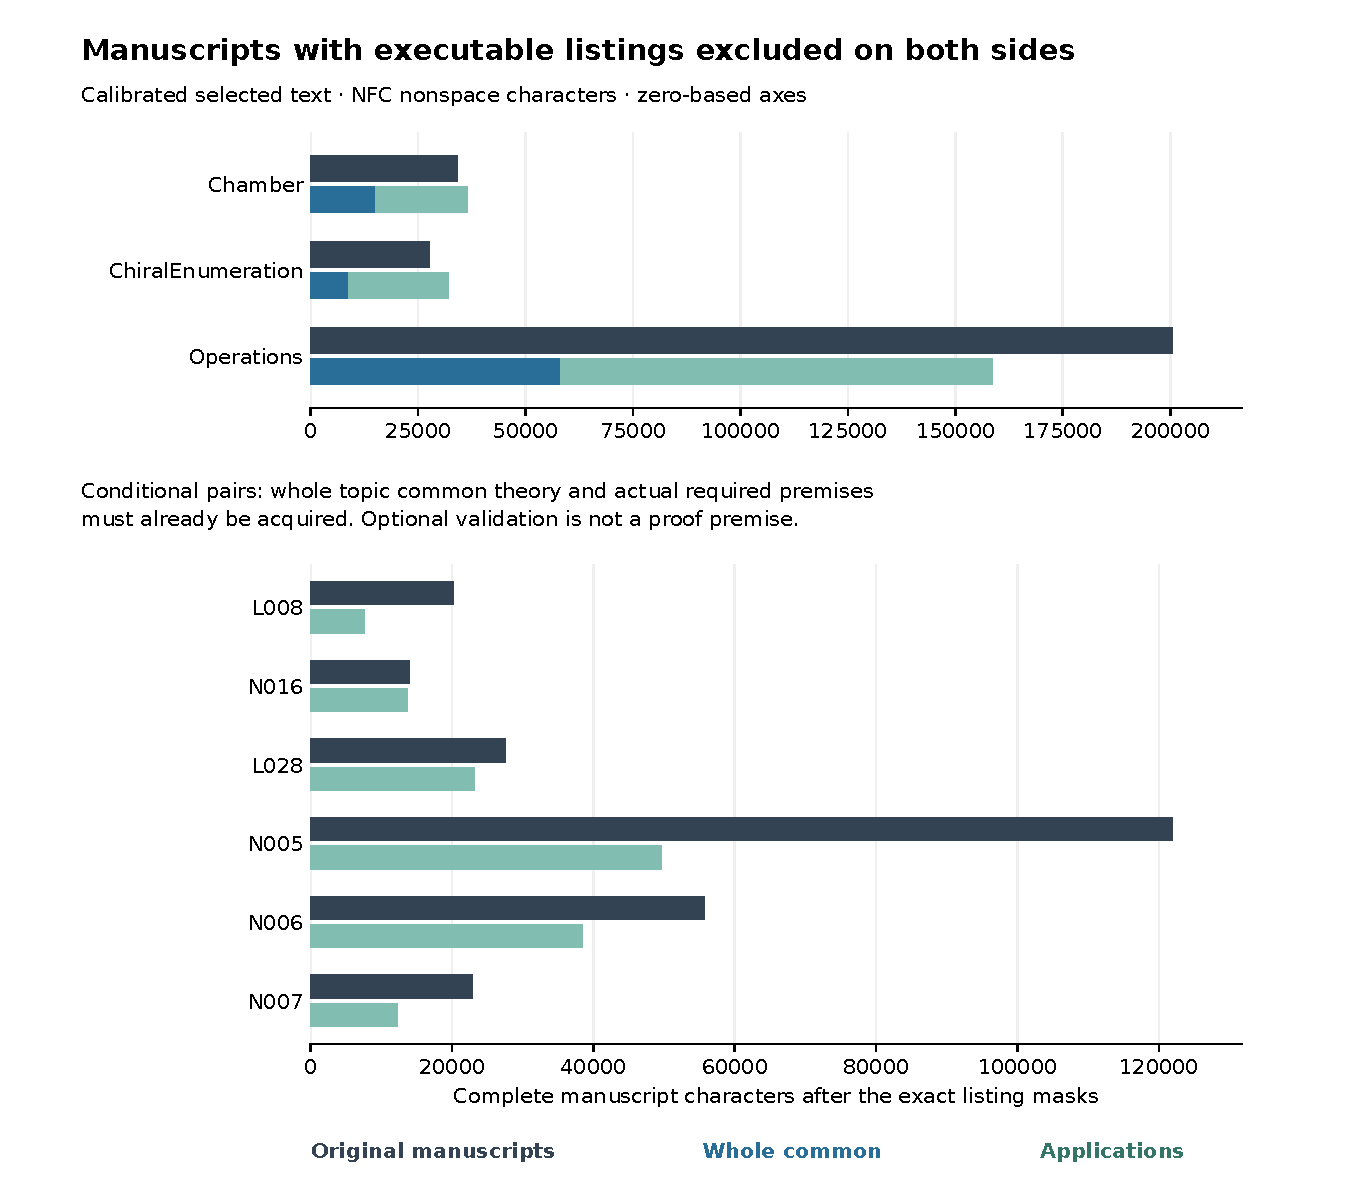
\includegraphics[width=\textwidth]{costs.pdf}\end{center}
The graphs show complete manuscript costs with axes starting at zero. Common theory is the blue portion of every whole-topic replacement bar; complete applications form the remaining portion. The conditional graph omits the already acquired common cost only under its stated acquisition condition. Required software and outside results remain separately disclosed, not treated as free or relabeled optional.

\textbf{What the masks exclude.} L008 has three Magma functions on physical pages 8--10, including literal program comments. L028 has three enumeration functions/procedure on pages 9--12; Lemma 4.5 and its entire proof, surrounding algorithm descriptions and Section 4.3 remain counted. N006 has one McL pseudocode block on page 20; the group construction, intersection-property definition, halving argument and conclusion remain counted. Twelve page-local chunks avoid all running headers and page numbers. The eleven replacement listing masks are empty.
\newpage
\textbf{Sensitivity and unchanged evidence.} All 600 accepted input cells are reused without re-extraction. Five hundred are unchanged, including every replacement cost. Each topic has the original three variants, two normalizations and five units. The complete 270 standard fractions and 40 additional Operations text-only fractions are supplied as exact integer fractions in JSON and CSV.
\begin{center}\begin{tabular}{lrr}\toprule
Whole topic, 30 standard coordinates & Minimum & Maximum\\\midrule
Chamber & 0.887879 & 1.027120\\
ChiralEnumeration & 0.862259 & 1.053323\\
Operations & 1.207971 & 1.421848\\
\bottomrule\end{tabular}\end{center}
These ranges disclose sensitivity; the primary coordinate was fixed before evaluation and is not selected from the range. Raw extraction, exact-furniture selection and calibrated selection remain distinct.

\textbf{Operations: text-only graphical sensitivity.}
\begin{center}\small\begin{tabular}{lrrr}\toprule
Unit & Originals & Whole replacement & Factor\\\midrule
NFC: Whitespace tokens & 47,076 & 34,582 & 1.361286\\
NFC: Alphanumeric units & 47,584 & 33,809 & 1.407436\\
NFC: Nonspace characters & 200,052 & 158,594 & 1.261410\\
NFC: Collapsed-space characters & 247,125 & 193,170 & 1.279314\\
NFC: Collapsed UTF-8 bytes & 261,672 & 216,381 & 1.209311\\
NFKC: Whitespace tokens & 47,168 & 34,582 & 1.363947\\
NFKC: Alphanumeric units & 47,584 & 33,809 & 1.407436\\
NFKC: Nonspace characters & 200,052 & 158,641 & 1.261036\\
NFKC: Collapsed-space characters & 247,217 & 193,217 & 1.279479\\
NFKC: Collapsed UTF-8 bytes & 261,098 & 197,152 & 1.324349\\
\bottomrule\end{tabular}\end{center}
This alternative replaces only previously bound graphical-proxy events by separators and applies the same listing masks. It does not remove ordinary labels or measure full diagram geometry. The original graphical-proxy sensitivity, font maps, physical pages and all scientific editions are unchanged. Full graphics, external proof costs, historical software and complete formalization costs remain unknown, not zero.

\textbf{Whole software remains visible.} The 46 exact files remain bound: Chamber's two mathematical/validation programs, three drivers and three partial formal files; ChiralEnumeration's three programs, driver and partial formal file; Operations' 23 mathematical/validation files, two required decoding drivers, five operational drivers and three partial formal files. Required and optional roles are unchanged. Complete installed/Atlas data and retained catalogue assumptions remain in the inherited inventory; no representation bytes or witness prerequisites were discarded. Partial printed appendices do not become a new full Operations software route.

The numerical author independently reviewed the new listing-mask inputs but did not author them. This arithmetic still requires distinct review. Earlier counts and comparisons remain immutable historical observations; this packet supplies a proposed successor boundary and does not rewrite earlier artifacts or the public catalogue.
\end{document}
